\documentclass[a4paper,12pt]{article}

\usepackage{graphicx}

\usepackage{graphicx}
\usepackage{geometry} % Modificar márgenes
\geometry{ % Especificación modificación márgenes
    a4paper,
    left=2cm,
    right=2cm,
    top=2cm,
    bottom=2cm
}
\usepackage[utf8]{inputenc}
\usepackage[spanish]{babel} % Paquete para escritura en español
\usepackage{float} % Etiqueta 'H' (mayus) en figuras (imágenes)
\usepackage{array} % Padding en tablas
\usepackage{url} % Etiqueta url en .bib
\usepackage{booktabs} % Manejo de caudros (tablas)
\usepackage[T1]{fontenc}    % Codificación de fuentes
\usepackage{csquotes}       % Paquete para comillas tipográficas

\begin{document}

\section{Objetivo}
Que el alumno conozca los principales aspectos teóricos y prácticos de las colecciones y sus aplicaciones en el lenguaje de programación Java, así mismo que ponga en práctica los conceptos básicos de la programación orientada a objetos.

\section{Introducción}

Las colecciones en Java son herramientas fundamentales en el desarrollo de software, especialmente en el ámbito de la ingeniería de software. Estas colecciones son conjuntos de objetos que permiten el almacenamiento, manipulación y gestión eficiente de datos en programas Java.

\section{¿Qué son las colecciones en Java?}

Las colecciones en Java son conjuntos de objetos que permiten el almacenamiento, manipulación y gestión eficiente de datos en programas escritos en Java. Estas colecciones forman parte del Java Collections Framework (JCF) como se puede ver en la Figura 1, una biblioteca estándar incluida en el lenguaje de programación Java. El JCF ofrece una amplia gama de interfaces y clases predefinidas que permiten trabajar con diferentes tipos de estructuras de datos, como listas, conjuntos y mapas.

En esencia, las colecciones en Java nos proporcionan herramientas para almacenar y organizar grupos de elementos relacionados de manera eficiente. Por ejemplo, podemos utilizar una lista para almacenar una secuencia ordenada de elementos, un conjunto para almacenar elementos únicos sin duplicados, o un mapa para almacenar pares clave-valor.

La inclusión de las colecciones en el JCF facilita el desarrollo de aplicaciones Java al proporcionar implementaciones eficientes y optimizadas de estructuras de datos comunes. Esto permite a los programadores centrarse en la lógica de la aplicación en lugar de tener que implementar manualmente las estructuras de datos subyacentes.

Además, el JCF ofrece operaciones y algoritmos comunes para trabajar con colecciones, como agregar elementos, eliminar elementos, buscar elementos, ordenar colecciones y realizar otras operaciones de manipulación de datos. Esto simplifica el proceso de desarrollo y mejora la coherencia y la eficiencia del código.

\section{Principales colecciones en Java}

La jerarquía de colecciones en Java se establece de manera que cada nivel proporciona un conjunto específico de funcionalidades y comportamientos para manejar grupos de elementos de manera eficiente.

\subsection{Collection}

En la cima de esta jerarquía se encuentra la interfaz Collection, que sirve como la base para todas las colecciones en Java. Esta interfaz define operaciones comunes que se aplican a cualquier colección, como agregar, eliminar y comprobar la presencia de elementos.

Una colección representa un grupo de objetos, conocidos como elementos. Algunas colecciones permiten elementos duplicados y otras no. Algunas están ordenadas y otras desordenadas. El JDK no proporciona ninguna implementación directa de esta interfaz, sino que proporciona implementaciones de subinterfaces más específicas. Esta interfaz se utiliza normalmente para pasar colecciones y manipularlas cuando se desea la máxima generalidad. \cite{collection}

\subsection{Set}

Los Sets en Java constituyen una colección que no permite elementos duplicados, lo que significa que cada elemento es único en el conjunto. Estos conjuntos utilizan los métodos equals y hashCode para determinar la duplicidad de los elementos. Una implementación común de Sets es HashSet, que almacena los elementos en una tabla hash para permitir un acceso rápido y eficiente a los elementos.

Se debe tener cuidado de utilizar objetos mutables como elementos establecidos, pues el comportamiento de un conjunto no se especifica si el valor de un objeto se cambia de una manera en la que afecta comparaciones entre iguales mientras el objeto es un elemento del conjunto. Un caso especial de esta prohibición es que no está permitido que un conjunto se contenga a sí mismo como elemento.\cite{set}

\subsection{Map}

Por otro lado, los Maps en Java son estructuras que asocian claves con valores, creando pares clave-valor únicos. Esto implica que no puede haber claves duplicadas en un Map. HashMap es una implementación común de Map que utiliza una tabla hash internamente para almacenar los pares clave-valor, lo que proporciona un acceso rápido a los datos. Por otro lado, TreeMap es otra implementación de Map que utiliza una estructura de árbol de búsqueda para mantener las claves ordenadas.

Proporciona tres vistas de colección, permitiendo ver el contenido de un mapa como un conjunto de claves, una colección de valores, o un conjunto de asignaciones de valores-clave.\cite{map}

\subsection{List}

Además, las Lists en Java representan colecciones ordenadas de elementos donde se permite la duplicación de elementos y se mantiene el orden de inserción. ArrayList es una implementación común de List que almacena elementos en un arreglo dinámico, lo que permite un acceso rápido a los elementos mediante índices. Por otro lado, LinkedList es otra implementación de List que utiliza una lista doblemente enlazada, ofreciendo un rendimiento eficiente para la inserción y eliminación de elementos en cualquier posición. Estas colecciones en Java proporcionan una base sólida para el desarrollo de aplicaciones eficientes y escalables.

\subsection{Queue}

Otra subinterfaz importante es Queue, que representa una colección en la que los elementos se insertan en un extremo y se eliminan del otro extremo siguiendo el principio de FIFO (\textit{First-In, First-Out}). Esto la hace adecuada para implementaciones de colas, como \textit{PriorityQueue}.

Una colección diseñada para manejar elementos antes de su procesamiento. Además de las operaciones básicas de recopilación, las colas proporcionan operaciones adicionales de inserción, extracción e inspección. \cite{queue}

\begin{figure}[ht]
    \centering
    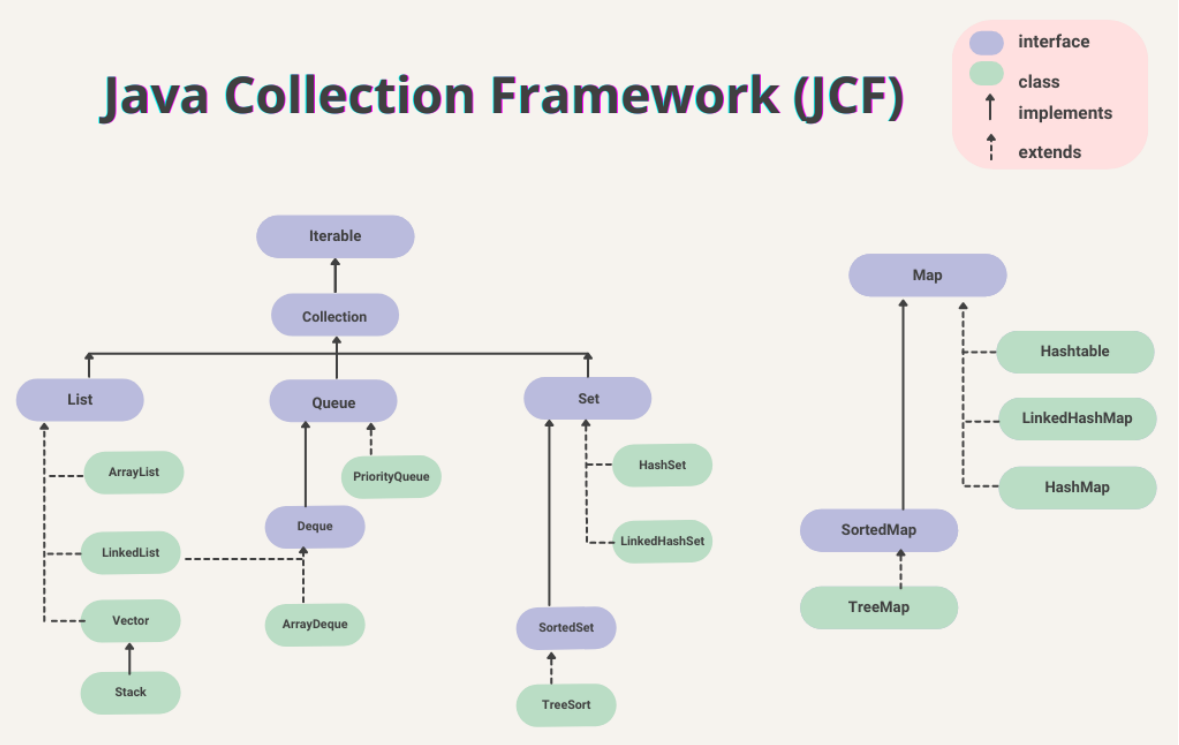
\includegraphics[width=.9\textwidth]{media/java_collection_framework.PNG}
    \caption{Java Collection Framework. \cite{nieva-2023}}
    \label{fig:enter-label}
\end{figure}

\section{Implementaciones (clases)}

Las clases que implementan las interfaces de colecciones en Java ofrecen funcionalidades específicas para diferentes tipos de almacenamiento y manipulación de datos.

Además de las interfaces, también hay clases concretas que implementan estas interfaces y proporcionan funcionalidades específicas. Por ejemplo, ArrayList y LinkedList son implementaciones de la interfaz List, mientras que HashSet y TreeSet son implementaciones de la interfaz Set. HashMap y TreeMap son implementaciones de la interfaz Map, que representa una colección de pares clave-valor.

\subsection{ArrayList}

El ArrayList es una de las implementaciones más utilizadas de la interfaz List, que almacena los elementos en un arreglo dinámico. Esto permite un acceso rápido a los elementos mediante índices, aunque las operaciones de inserción y eliminación pueden ser costosas en términos de rendimiento, especialmente para grandes conjuntos de datos.

Implementa todas las operaciones de lista opcionales y permite todos los elementos, incluido el nulo. Además de implementar la interfaz List, esta clase proporciona métodos para manipular el tamaño de la matriz que se utiliza internamente para almacenar la lista. \cite{array_list}

Cada instancia de ArrayList tiene una capacidad. La capacidad es el tamaño de la matriz utilizada para almacenar los elementos de la lista. Siempre es al menos tan grande como el tamaño de la lista. A medida que se agregan elementos, su capacidad crece automáticamente.  \cite{array_list}

Es importante mencionar que esta implementación no está sincronizada, lo que significa que, si varios subprocesos acceden a una instancia de ArrayList simultáneamente y al menos uno de ellos realiza cualquier operación que agregue o elimine uno o más elementos, o cambia explícitamente el tamaño de la matriz (modificaciones estructurales), se debe sincronizar externamente. \cite{array_list}

\subsection{LinkedList}

Por otro lado, LinkedList es otra implementación de la interfaz List que utiliza una lista doblemente enlazada. Si bien ofrece un rendimiento eficiente para la inserción y eliminación de elementos en cualquier posición, acceder a elementos por índice puede ser menos eficiente que en ArrayList.

Todas las operaciones se realizan como se podría esperar de una lista doblemente enlazada. Las operaciones que indexan la lista recorrerán la lista desde el principio o el final, lo que esté más cerca del índice especificado.\cite{linked_list} De manera exactamente igual a como sucede con ArrayList, la implementación no está sincronizada y se debe sincronizar externamente de realizar modificaciones estructurales un subproceso.

\subsection{HashSet}

HashSet es una implementación de la interfaz Set que almacena elementos en una tabla hash (en realidad es una instancia de HashMap), lo que garantiza un acceso rápido a los elementos y la prohibición de elementos duplicados. Esta implementación es ideal cuando se necesita una colección sin elementos duplicados y el orden de los elementos no es importante, pues no garantiza que el orden se mantendrá constante en el tiempo, ni en cuanto al orden de iteración del conjunto.

Permite el elemento nulo y ofrece un rendimiento constante para las operaciones básicas (agregar, eliminar, contener y dimensionar), suponiendo que la función hash disperse los elementos adecuadamente entre los depósitos (\textit{bucket}). De manera exactamente igual a como sucede con LinkedList y ArrayList, la implementación no está sincronizada y se debe sincronizar externamente de realizar modificaciones estructurales un subproceso. \cite{hash_set}

\subsection{TreeSet}

TreeSet, por otro lado, es otra implementación de la interfaz Set que almacena elementos en un árbol de búsqueda ordenado. Esto garantiza que los elementos se mantengan ordenados según un criterio especificado, lo que puede ser útil en ciertas situaciones donde se necesita mantener un orden específico en la colección.

Los elementos se ordenan utilizando su orden natural o mediante un Comparador proporcionado en el momento de la cración establecido, según el constructor que se utilice. Esta implementación proporciona un costo de tiempo $log(n)$ garantizado para las operaciones básicas (agregar, eliminar y verificar existencia). \cite{tree_set}

\subsection{HashMap}

Para las implementaciones de la interfaz Map, HashMap es una implementación común que utiliza una tabla hash para almacenar pares clave-valor, lo que permite un acceso rápido a los valores a través de las claves a cambio de no ofrecer garantías en cuanto al orden del mapa.

Una instancia de HashMap tiene dos parámetros que afectan su rendimiento: capacidad inicial y factor de carga. La capacidad es la cantidad de depósitos en la tabla hash y la capacidad inicial es simplemente la capacidad en el momento en que se crea la tabla hash. El factor de carga es una medida de qué tan llena se permite que esté la tabla hash antes de que su capacidad aumente automáticamente. Cuando el número de entradas en la tabla hash excede el producto del factor de carga y la capacidad actual, la tabla hash se repite (es decir, se reconstruyen las estructuras de datos internas) para que la tabla hash tenga aproximadamente el doble de la cantidad de depósitos. \cite{hash_map}

\subsection{TreeMap}

Por otro lado, TreeMap es otra implementación de la interfaz Map que utiliza un árbol de búsqueda para mantener las claves ordenadas, lo que puede ser útil en situaciones donde se necesita mantener un orden específico en las claves.

El mapa se ordena según el orden natural de sus claves o mediante un comparador proporcionado en el momento de la creación del mapa, según el constructor que se utilice.
Esta implementación proporciona un costo de tiempo de $log(n)$ garantizado para las operaciones contiene clave, obtener, colocar y eliminar. \cite{tree_map}

Hay que tener en cuenta que esta implementación no está sincronizada. Si varios subprocesos acceden a un mapa al mismo tiempo y al menos uno de los subprocesos modifica el mapa estructuralmente, debe sincronizarse externamente. \cite{tree_map}

\section{Principales diferencias entre las implementaciones}

Es importante comprender las diferencias fundamentales entre las implementaciones de colecciones en Java, ya que estas diferencias afectan el rendimiento y la eficiencia de nuestros programas.

En primer lugar, en el caso de ArrayList y LinkedList, la diferencia radica en cómo se almacenan los elementos. ArrayList utiliza un arreglo dinámico, lo que permite un acceso rápido a los elementos mediante índices, pero las inserciones y eliminaciones pueden ser costosas. Por otro lado, LinkedList utiliza una lista doblemente enlazada, lo que facilita las inserciones y eliminaciones en cualquier posición, pero puede ser menos eficiente para el acceso aleatorio.

En cuanto a HashSet y TreeSet, la distinción principal está en cómo se organizan los elementos y se garantiza la unicidad. HashSet utiliza una tabla hash, ofreciendo un acceso rápido a los elementos y prohibiendo duplicados, pero no garantiza ningún orden particular de los elementos. Por otro lado, TreeSet utiliza un árbol de búsqueda, lo que garantiza que los elementos se mantengan ordenados y únicos, aunque puede ser un poco más lento debido a las operaciones de ordenación internas.

Por último, en el caso de HashMap y TreeMap, la diferencia principal radica en la organización de las claves. HashMap utiliza una tabla hash para un acceso rápido a los valores a través de las claves, sin garantizar un orden particular de las claves. Por otro lado, TreeMap utiliza un árbol de búsqueda para mantener las claves ordenadas, garantizando un orden específico de las claves, pero potencialmente con un rendimiento ligeramente inferior debido a las operaciones de ordenación.


\section{Aspectos cruciales para la implementación de colecciones en Java en la resolución eficiente de problemas}

\subsection{Análisis de requisitos}

Antes de empezar a resolver un problema es importante entender qué tipo de datos necesitamos manejar. ¿Necesitamos una lista que mantenga un orden específico? ¿O tal vez un conjunto donde no se permitan elementos duplicados? Hay diferentes tipos de colecciones en Java para diferentes necesidades. Por ejemplo, si queremos buscar elementos de manera rápida podríamos elegir HashSet.

\begin{figure}[ht]
    \centering
    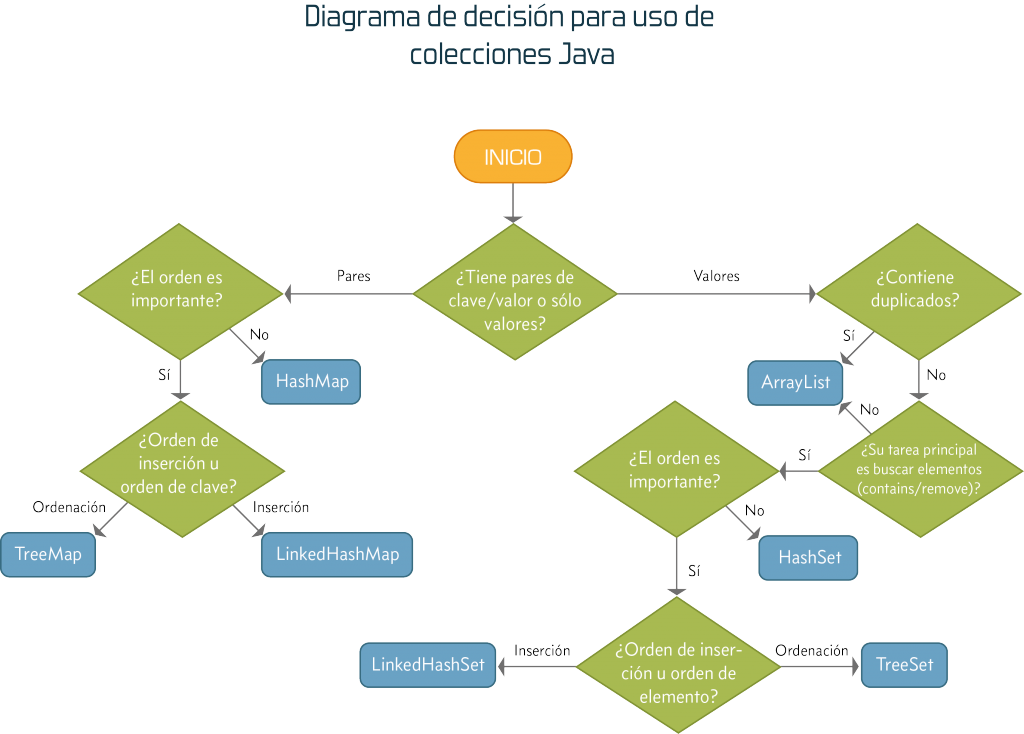
\includegraphics[width=.9\textwidth]{media/diagrama_decision_uso_de_colecciones.png}
    \caption{Diagrama de decisión para el uso de colecciones en Java. \cite{amor-2020}}
    \label{fig:diagrama_decision_colecciones}
\end{figure}

\subsection{Eficiencia temporal y espacial}

Cuando elijamos una colección, debemos pensar en cómo funcionará en términos de velocidad y espacio. ¿Qué tan rápido será para agregar, buscar o eliminar elementos? ¿Cuánta memoria utilizará? Por ejemplo, si usamos ArrayList, podemos acceder a los elementos rápidamente, pero si necesitamos agregar o eliminar elementos con frecuencia, LinkedList podría ser mejor.

\subsection{Manejo de duplicados}

A veces, no queremos que haya elementos repetidos en nuestra colección. En ese caso, podemos usar un conjunto (Set). Si necesitamos que los elementos se mantengan en un orden específico, podríamos usar LinkedHashSet.

\subsection{Iteración y recorrido}

Cuando necesitamos recorrer una colección, es importante hacerlo de manera eficiente. Podemos usar bucles especiales como el for-each. Pero debemos recordar que algunas colecciones, como HashSet, no garantizan un orden específico.

\subsection{Claves y valores en mapas}

Si necesitamos asociar claves con valores, podemos usar un mapa (Map). Es importante elegir claves únicas y significativas. Por ejemplo, si estamos usando HashMap, debemos asegurarnos de que nuestras claves sean únicas.

\subsection{Manejo de excepciones}

Al escribir código, siempre debemos estar preparados para manejar errores. Es importante considerar posibles excepciones como \textit{NullPointerException} o \textit{ConcurrentModificationException} y usar bloques \textit{try-catch} para manejarlas.

\subsection{Documentación y comentarios}

Finalmente, al escribir código es útil documentar lo que estamos haciendo y por qué lo estamos haciendo de esa manera. Esto ayuda a otros a entender nuestro código y también a nosotros mismos en el futuro. Es importante agregar comentarios para explicar nuestras decisiones de diseño.

\section{Análisis del programa}

\subsection{Admin.java}
Dentro de la clase “Análisis.java” un administrador puede realizar diversas acciones como 
registrar alumnos, docentes, asignaturas, y abrir grupos. La clase contiene un método 
estático “iniciar()” que sirve como punto de entrada, presentando un menú de opciones al 
usuario y ejecutando las acciones correspondientes según la selección. Se emplea la clase 
Scanner para capturar la entrada del usuario desde la consola.
El menú de opciones ofrece al administrador diez acciones diferentes, desde registrar 
alumnos hasta cerrar sesión. Para cada opción, se utiliza una estructura de control switch-case que dirige el flujo del programa hacia el método adecuado en la clase Sistema.
El caso “nuevoGrupo()” permite al administrador abrir un nuevo grupo, solicitando la clave de 
la asignatura y el RFC del docente. Una vez proporcionados estos datos, el método llama a la 
función “abrirGrupo()” de la clase Sistema para crear el grupo correspondiente.
El programa incluye un mecanismo para manejar situaciones donde el usuario introduce una 
opción no válida. En tal caso, se imprime un mensaje de error y se llama recursivamente al 
método “iniciar()” para volver a mostrar el menú de opciones.

\subsection{Alumnos.java}
La clase llamada “Alumnos.java”, representa a los estudiantes de la F.I. Cada instancia de 
esta clase almacena información como el número de cuenta, nombre, contraseña y los 
grupos en los que está inscrito el alumno.
El método “opciones()” es el punto de entrada principal para los alumnos, mostrando un 
menú de opciones que permite al estudiante realizar diversas acciones, como ver las 
materias inscritas, mostrar grupos por clave o nombre de asignatura, dar de alta o baja un 
grupo, cambiar de grupo o cerrar sesión. Este método utiliza un objeto Scanner para capturar 
la entrada del usuario desde la consola.
Para cada opción del menú, se emplea una estructura switch-case para dirigir el flujo del 
programa hacia el método correspondiente. Por ejemplo, el caso 
“imprimirMateriasInscritas()” muestra las materias en las que está inscrito el alumno, 
mientras que los casos “inscribir()”, “desinscribir()” y “cambiarGrupo()” permiten al alumno 
interactuar con los grupos de asignaturas.
El método “inscribir()” solicita al alumno la clave de la asignatura y el número de grupo al que 
desea inscribirse, verificando la disponibilidad de grupos para esa asignatura. Similarmente,
“desinscribir()” y “cambiarGrupo()” permiten al alumno darse de baja de un grupo o cambiar 
de grupo respectivamente, con validaciones para asegurar que la acción sea válida.

\subsection{Grupo.java}
La clase “Grupos.java”, representa los grupos de estudiantes inscritos en una asignatura. 
Cada instancia de esta clase almacena información como el número de alumnos inscritos, el 
número de grupo, y el nombre del profesor a cargo.
La clase cuenta con métodos getter y setter para acceder y modificar los atributos de los 
grupos, como el número de grupo, el número de alumnos inscritos, la lista de alumnos 
inscritos y el nombre del profesor.
La lista de alumnos inscritos se implementa utilizando una LinkedList, lo que permite 
almacenar eficientemente un número variable de alumnos en cada grupo.

\subsection{Materias.java}
La clase “Materias.java”, representa las asignaturas impartidas en la F.I. Cada instancia de 
esta clase almacena información como la clave de la asignatura, el nombre y una lista de 
grupos asociados a esa asignatura.
La clase cuenta con constructores que permiten inicializar una asignatura con su nombre y 
opcionalmente con su clave y lista de grupos. También incluye métodos getter y setter para 
acceder y modificar los atributos de la asignatura, como el nombre, la clave y la lista de 
grupos.
El método “generarClave()” se encarga de generar una clave única para la asignatura 
utilizando el primer carácter del nombre y un número consecutivo basado en la cantidad total 
de asignaturas existentes en el sistema. Esta clave se calcula mediante una fórmula que 
combina el valor numérico del primer carácter del nombre con un valor constante y el 
número total de asignaturas.

\subsection{Profesores.java}
La clase “Profesores.java”, representa a todos los profesores que imparten clase en la F.I. 
Cada instancia de esta clase almacena información como el nombre del profesor, su usuario, 
la clave de acceso al sistema, y una lista de grupos que el profesor imparte.
El constructor de la clase permite inicializar un profesor con su usuario, nombre y clave de 
acceso al sistema.
La clase cuenta con métodos getter y setter para acceder y modificar los atributos del 
profesor, como el nombre, la clave y la lista de grupos que imparte.
El método “opciones()” es el punto de entrada principal para los profesores, mostrando un 
menú de opciones que permite al profesor realizar diversas acciones, como mostrar los 
grupos que imparte, mostrar grupos por clave o nombre de asignatura, solicitar dar grupo de 
una asignatura, ver la lista de alumnos o cerrar sesión.
Para cada opción del menú, se emplea una estructura switch-case para dirigir el flujo del 
programa hacia el método correspondiente. Por ejemplo, el caso 
“mostrarGruposImpartidos()” muestra los grupos que el profesor imparte, mientras que el 
caso “solicitarImpartir()” permite al profesor solicitar impartir una asignatura.

\subsection{SistemaDeInscripciones.java}
La clase “Sistemadeinscripcion.java”, es un punto de entrada principal para el sistema de 
inscripción. La clase contiene un método estático “main()” que se encarga de llamar al 
método estático “inicioSesion()” de la clase Sistema.
El método “main()” es el punto de entrada principal de cualquier programa Java. En este caso, 
simplemente llama al método “inicioSesion()” de la clase Sistema.

\subsection{Sistema.java}
“Sistema.java”, es el núcleo del sistema de inscripción. Esta clase contiene múltiples 
atributos estáticos, como tablas hash y listas, para almacenar información sobre 
asignaturas, alumnos y profesores.
El método “inicioSesion()” es el punto de entrada principal del sistema. Permite a los 
usuarios iniciar sesión como alumno, docente o administrador, y luego los redirige a las 
opciones correspondientes.
Para los alumnos, el método “iniciarAlumno()” maneja las opciones de inicio de sesión y 
registro. El método “ingresarAlumno()” permite a los alumnos ingresar al sistema con su 
número de cuenta y contraseña, mientras que “crearAlumno()” permite registrar una nueva 
cuenta de alumno.
Para los docentes, el proceso es similar. El método” iniciarDocente()” maneja las opciones de 
inicio de sesión y registro. “ingresarDocente()” permite a los docentes ingresar al sistema con 
su RFC y contraseña, mientras que “crearDocente()” permite registrar una nueva cuenta de 
docente.
El método iniciarAdmin() permite al administrador iniciar sesión utilizando una contraseña 
predefinida y luego acceder a las funciones de administración del sistema.
Además, hay métodos para imprimir información sobre alumnos, docentes y asignaturas, así 
como para crear nuevas asignaturas y grupos, inscribir y dar de baja alumnos de grupos, y 
cambiar grupos de asignaturas para los alumnos.

\section{Conclusiones}

\subsection{Cabrera Rojas Oscar}

Lorem ipsum dolor sit amet...

\subsection{Espejel Ornelas Irvin Giovanni}

Las colecciones en Java son componentes esenciales en el desarrollo de software, ya que nos permiten manejar eficientemente grupos de elementos relacionados. Desde listas hasta conjuntos y mapas, estas estructuras nos brindan la flexibilidad y funcionalidad necesarias para abordar una amplia gama de problemas de programación. 

Es crucial comprender las diferencias entre las diferentes implementaciones de colecciones, así como sus ventajas y limitaciones. Cada tipo de colección tiene su propósito y ofrece características específicas que pueden afectar el rendimiento y la eficiencia de nuestros programas. 

Además, la elección de la implementación de colección adecuada depende en gran medida de los requisitos del problema que estamos tratando de resolver. Ya sea que necesitemos mantener un orden específico, evitar duplicados o asociar claves con valores, es importante seleccionar la estructura de datos más apropiada para nuestras necesidades.

\subsection{López Katt Edmundo}

Lorem ipsum dolor sit amet...

\bibliographystyle{acm}
\bibliography{main, api}

\end{document}

